\section{Background}
In this section some basics concepts related to the human walking are introduced. Later they will
be applied to the robot walking.
\subsection{Locomotion in human being}
The \emph{gait cycle} is defined as the time between two successive foot contact of the same limbs,
it can be divided in two phases, the \emph{Stance Phase}  and the \emph{Swing phase}.
For analyzing gait cycle one foot is taken as reference and its movements studied.
The Stance phase is the part of a gait cycle during which the foot remains in contact with the
ground, it constitutes about the $60\%$ of the gait cycle. In this phase five parts can be
distinguished:
\begin{itemize}
\item [-]\emph{Initial contact}: Instant when the foot contacts the ground;
\item [-]\emph{Loading response}: Time period between the initial contact phase and the instant
  when the other foot lifts the ground;
\item [-]\emph{Mid stance}: Time interval from the end of the Loading response phase to the time
  when both ankles are aligned in the frontal plane;
\item[-]\emph{Terminal stance}: Period from ankles alignment to the contact of the swinging foot;
\item[-]\emph{Pre swing}: Time interval between the end of the terminal stance phase and the instant
  when the foot lifts from the ground.
\end{itemize}
The Swing phase is the phase of the gait during which the reference foot swings. It takes about $40\%$ of the gait cycle and it can be distinguished in three parts:
\begin{itemize}
\item [-]\emph{Initial swing}: Phase during which the reference foot is lifted from the ground
  to position of maximum knee flexion;
\item [-]\emph{Mid swing}: Time period between the maximum knee flexion and the instant when the tibia reaches the vertical position;
\item[-]\emph{Terminal swing}: Following vertical tibia position to just prior to initial contact.
\end{itemize}
Last but not least the concepts of Double and Single support are introduced. The first one refers to
the period during which boot feet are in contact with the ground while the other refers to interval when only one foot is in contact with the ground.
\par
In Figure \ref{fig:gait-cycle} all the phases described above are shown. For each phase the type of support (single or double) is specified.
\begin{figure}[!ht]
  \centering
  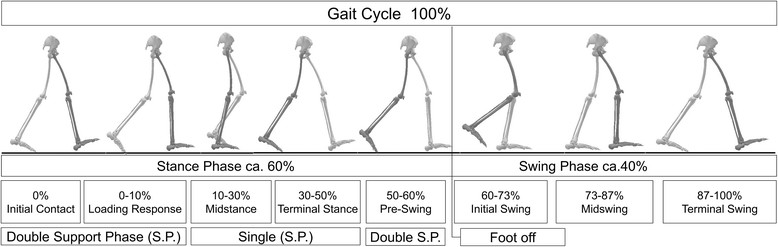
\includegraphics[scale=0.45]{gait-cycle.png}
  \caption{Classification of a human gait cycle. Image taken from \cite{Merker2015}. \label{fig:gait-cycle}}
\end{figure}
\par
In the following subsection the concepts described will be applied to the robot walking.
\subsection{Locomotion in robotic systems}
In robot locomotion the gait cycle described in the above section is simplified,
and the phases described are condensed in more general groups.
The walking task can be easy summarize using the \emph{walking cycle}
(Figure \ref{fig:walking_fsm}), it embeds all the phases of the human locomotion
shown in the Figure \ref{fig:gait-cycle}. 
\begin{figure}[!ht]
  \centering
  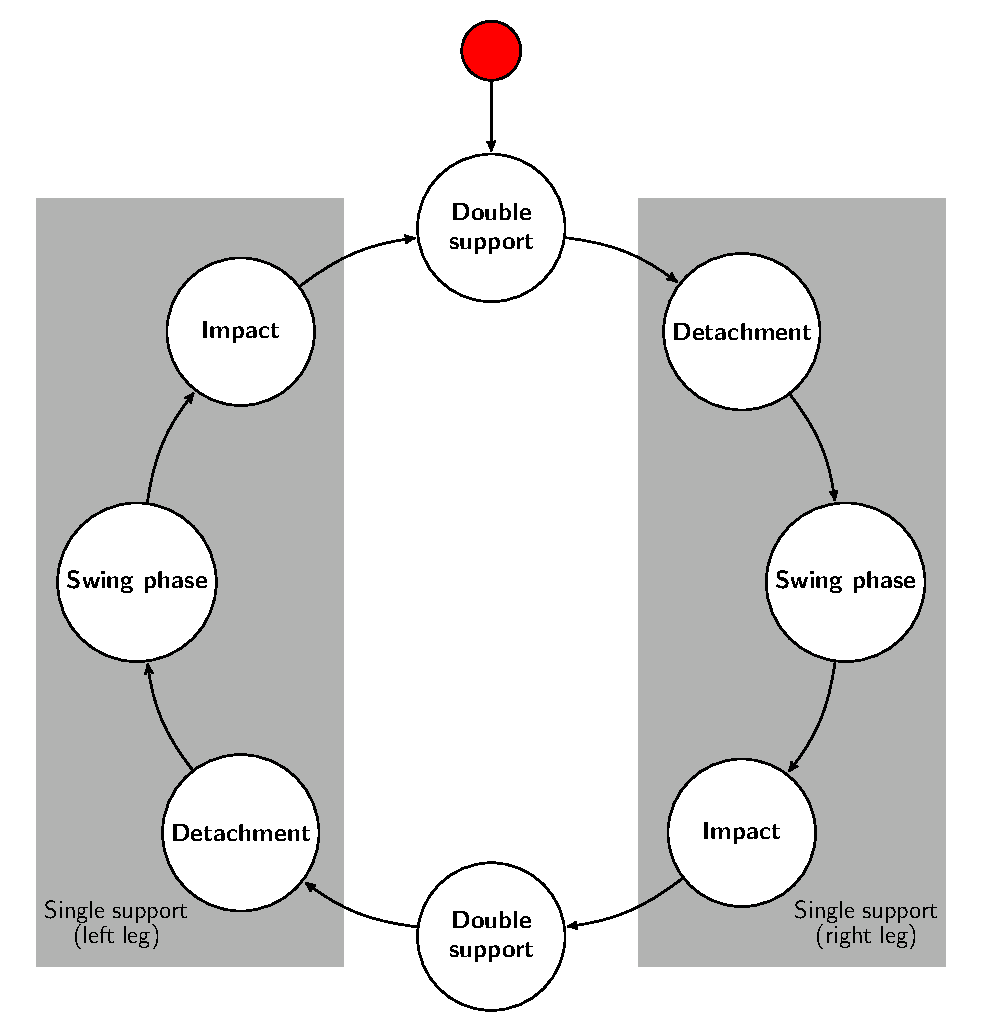
\includegraphics[scale=0.46]{walking_fsm}
  \caption{Walking cycle state machine. \label{fig:walking_fsm}}
\end{figure}
\par
The cycle can be split in two main phases, the Double support and the Single support ones.
The first one embeds the initial contact, the loading response and the pre swing phases while the
single support phase embeds the others.
During the SS phase the movement of the swing foot 
is usually split in three sub-phases, \emph{detachment}, \emph{swing} and \emph{impact}.
More detailed:
\begin{itemize}
\item[-]\emph{Detachment}: Instant when the foot lifts from the ground;
\item[-]\emph{Swing}: this phase embeds the Initial swing, the mid swing and the terminal swing
  stages of the human walking;
\item[-]\emph{Impact}: Instant when the foot contacts the ground.
\end{itemize}
In the following of this report only the single support phase is analyzed.

\subsection{Zero Momentum Point}
In order to derive a model for the robotic locomotion the \emph{Zero Momentum Point} concept
\cite{Vukobratovic1969} must be discussed.
In the following dissertation only the single support phase is considered and, in order to simplify the analysis, only the reference foot is considered.
\par
In the free body diagram of the reference foot (Fig \ref{fig:zmp_foot}) the influence of the
entire robot is replaced by the force applied to the point $A$
($\vec{F}_A$) and the torque relative to $A$ ($\vec{M}_A$) while the
total ground reaction consist on a force applied to the point $P$ ($\vec{R}$) and a torque
relative to $P$ ($\vec{M}$), finally the weight of the foot itself acts at its gravity center $G$.
\begin{figure}[!ht]
  \centering
  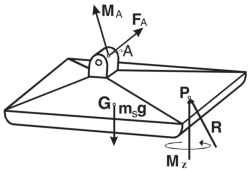
\includegraphics[scale=1.5]{zmp_foot}
  \caption{Free body diagram of the reference foot. Image edit from \cite{Vukobratov2004}. \label{fig:zmp_foot}}
\end{figure}
\par
The horizontal components of the reaction force $\vec{R}$ ($R_x$ and $R_y$) are 
the friction force necessary to balance the horizontal components of the force $\vec{F}_A$, while
the vertical component of the reaction torque $\vec{M}$ ($M_z$) represents moment generated by the
friction reaction forces and it balances the vertical component of the torque $\vec{M}_A$.
In the following, the reference foot is assumed in contact with the ground without sliding, therefore
the friction compensates the horizontal force components ($R_x$, $R_y$) and vertical reaction torque
($M_z$). The vertical reaction force $R_z$ compensates the vertical component of the force
$\vec{F}_A$ and the weight of the foot itself.  
\par
Finally it is very interesting to study the balancing of the horizontal component of the
torque $\vec{M_A}$ ($M_{A_x}$ and $M_{A_y}$). Because of the unilateral nature of the constraint between
the reference foot and the ground, these components can be only compensate by changing
the position of the point $P$ within the support polygon.
\par
In the Figure \ref{fig:zmp_foot_y} a simple planar case in sagittal plane is presented. In this
simple scenario the component $M_{A_x}$ is balanced by shifting the point $P$.
\begin{figure}[!ht]
  \centering
  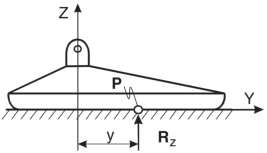
\includegraphics[scale=1.5]{zmp_foot_y}
  \caption{Example of a planar case. Image taken from \cite{Vukobratov2004}. \label{fig:zmp_foot_y}}
\end{figure}

It is important to note that all the time the reaction force $\vec{R}$ is within the support polygon
the ankle moment is full compensate by changing the position of the point $P$ and the horizontal
components of the interaction torque with the ground are zero. In the light of this statement in the
Figure \ref{fig:zmp_foot} only the component $M_z$ exists.
However, in the case which the sole is not large enough to allow the appropriate position of the
point $P$ the force $\vec{R}$ acts at the edge of the foot and the horizontal components $M_x$ and
$M_y$ are different from zero.
\par
The reasoning presented above can be summarized in the following principle \cite{Vukobratov2004}.
\begin{principle}
  The necessary and sufficient condition for the locomotion mechanism to be stable
  is that for the point $P$ on support polygon where the ground reaction force is acting
  \[
  M_x = 0 \quad M_y = 0
  \]
\end{principle}
\subsubsection{Zero Momentum Point evaluation}
In this section the position of the Zero Momentum Point is evaluated. It should be noted that the
prerequisite of the stability of the entire robot is the stability of the contact between the
reference foot and the ground. Thus for the supporting foot the following equations hold 
\[
\vec{R} + \vec{F}_A + m_s \vec{g} = \vec{0}
\]
\begin{equation}
  \label{eq:zmp_2_cardinal}
  \vec{OP} \times \vec{R} + m_s \vec{OG} \times \vec{g} + \vec{OA} \times \vec{F}_A + \vec{M}_A +
  \begin{bmatrix}
    0 \\
    0 \\
    M_z
  \end{bmatrix} = \vec{0}
\end{equation}
where $\vec{R}$, $M_z$, $\vec{F}_A$, $\vec{M}_A$ and $m_s$ are shown in Figure
\ref{fig:zmp_foot}, while $\vec{OP}$, $\vec{OG}$ and $\vec{OA}$ are respectively the position vector
from the origin of the coordinate system $O_{xyz}$ to the ground reaction force acting point ($P$),
CoM of the foot ($G$) and the ankle joint ($A$).
\par

Projecting the second cardinal equation (\ref{eq:zmp_2_cardinal}) onto the $z$-axis and placing the
origin of the reference system $O$ at $P$ (i.e. $O \equiv P$), $M_z$ can be evaluated
\[
M_z = M_{fr} = [-(\vec{M}_A + \vec{PA} + \vec{F}_A)]_z
\]
where $[\vec{v}]_z$ means $\langle \vec{v},\vec{e}_3 \rangle$.
\par
The projection of the equation (\ref{eq:zmp_2_cardinal}) onto the horizontal plane ($xy$-plane) gives
\[
\left[\vec{OP} \times \vec{R} + m_s \vec{OG} \times \vec{g} + \vec{OA} \times \vec{F}_A + \vec{M}_A\right]_{(x,y)} = \vec{0}
\]
placing the origin of the reference system $O$ at $P$ (i.e. $O \equiv P$) the following relation holds
\begin{equation}
  \label{eq:zmp_eq}
  \left[ m_s \vec{PG} \times \vec{g} + \vec{PA} \times \vec{F}_A + \vec{M}_A\right]_{(x,y)} = \vec{0}
\end{equation}
An intuitive understanding is obtained by setting $m_s = 0$ and $\vec{M}_A = \vec{0}$ in equation
(\ref{eq:zmp_eq})
\[
\left[\vec{PA} \times \vec{F}_A\right]_{(x,y)} = \vec{0}
\]
in this particular case $P$ is the point on the ground where the line of the action of $\vec{F}_A$
penetrates (Figure \ref{fig:zmp_foot_y_example}).
\begin{figure}[!ht]
  \centering
  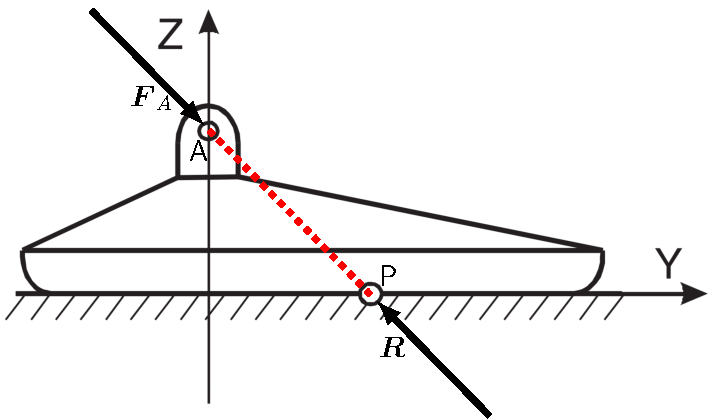
\includegraphics[scale=0.56]{zmp_foot_y_example}
  \caption{ZMP simple example. Image edit from \cite{Vukobratov2004}. \label{fig:zmp_foot_y_example}}
\end{figure}
The equation (\ref{eq:zmp_eq}) allows to evaluate the ZMP position. In order to understand if the robot
is in dynamic equilibrium the position of $P$ must be within the support polygon. However, in reality, the
point $P$ cannot exist outside the support polygon.
\par
The following principle holds:
\begin{principle}
  \label{principle:zmp}
  The position of the point $P$ is inside the convex hull of the foot support area ($\Omega$)
  IFF the robot is in dynamic equilibrium.
  \[
  P \in \Omega \longleftrightarrow \text{dyanamic equilibrium}
  \]
  \par
  However if the point $P \in \partial \Omega$ it is not possible to conclude on the stability of the robotic system.
  \par
  Where $\partial \Omega$ is the boundary of $\Omega$ (i.e. $\bar{\Omega} = \Omega \cup \partial \Omega$).
\end{principle}
Thus, in some case, the position of ZMP may not be an accurate criterion to distinguish between a
stable walk and an unstable one, to solve this problem a new concept must be introduced: the
Fictitious Zero Momentum Point, also know with the name of Foot Rotation Indicator (FRI)
\cite{Goswami1999}.

\subsection{Foot Rotation Indicator}
In order to solve the problem of the ZMP another point is introduced. The FRI point is a point on
the ground surface, within or outside the support polygon, where the ground reaction force $\vec{R}$
\emph{would} have to act in order to keep the foot stable.
In order to formally define the FRI point the entire robot must be taken into
account.
\par
The following dynamic equation holds 
\[
\vec{M} + \vec{OP} \times \vec{R} + \sum_{i=0}^{N-1} {\vec{OG}_i \times m_i \vec{g}} = \sum_{i=0}^{N-1}
\dot{\vec{H}}_{G_i} + \sum_{i=0}^{N-1} {\vec{OG}_i \times m_i \vec{a}_i}
\]
where $m_i$ is the mass, $G_i$ is the position of CoM, $\vec{H}_{G_i}$ is the angular momentum about the CoM and $\vec{a}_i$ is the CoM linear acceleration of the $i$-th link, while $\vec{M}$ and
$\vec{R}$ are define in the below section.
\par
Following the same steps of the ZMP evaluation the dynamic of the entire robot, except from
the reference foot, is completely represented by a force $\vec{F}_A$ and a torque $\vec{M}_A$.
\par
The dynamic equation of the foot is
\begin{equation}
  \label{eq:zmp_dyn_eq}
  \vec{M} + \vec{OP} \times \vec{R} + \vec{OG}_0 \times m_0 \vec{g} + \vec{M}_A + \vec{OA} \times \vec{F}_A  = \dot{\vec{H}}_{G_0} + \vec{OG}_0 \times m_i \vec{a}_0
\end{equation}
It important to note that the equation (\ref{eq:zmp_2_cardinal}) can be easily obtained from
\ref{eq:zmp_dyn_eq} by setting the dynamic terms to $\vec{0}$.
In the special case in which $O \equiv P$ where $P$ is the Center of pressure. the static
equilibrium of the foot becomes
\begin{equation}
  \label{eq:foot_equilibrium}
  \vec{M} + \vec{PG}_0 \times m_0 \vec{g} + \vec{M}_A + \vec{PA} \times \vec{F}_A = \vec{0}
\end{equation}
Projecting the equation (\ref{eq:foot_equilibrium}) onto the $xy$-plane the equation
(\ref{eq:zmp_eq}) is obtained and in the presence of unbalanced torque on the foot it
is not satisfied for any point inside the support polygon. However, the equation
can be solved by a point $F$ outside the convex hull
\begin{equation}
  \label{eq:fri_eq}
  \left [\vec{FG}_0 \times m_0 \vec{g} + \vec{M}_A + \vec{FA} \times \vec{F}_A \right]_{(x,y)} = \vec{0}
\end{equation}
In the following, the point $F$ will be called Foot Rotation Indicator (FRI) point.
An explicit solution of the equation (\ref{eq:fri_eq}) was find by Goswami \cite{Goswami1999};
the main idea is compute the ``dynamic of the robot without the foot''
\[
-\vec{M}_A - \vec{FA} \times \vec{F}_A + \sum_{i=1}^{N-1} {\vec{FG}_i \times m_i \vec{g}} = \sum_{i=1}^{N-1}
\dot{\vec{H}}_{G_i} + \sum_{i=1}^{N-1} {\vec{FG}_i \times m_i \vec{a}_i}
\]
considering only the tangential plane and using the equation (\ref{eq:fri_eq})
\[
\left[\vec{FG}_0 \times m_0 \vec{g} + \sum_{i=1}^{N-1}\vec{FG}_i \times m_i (\vec{g}-\vec{a}_i)\right]_{(x.y)} = \left[ \sum_{i=1}^{N-1} \dot{\vec{H}}_{G_i} \right]_{(x,y)}
\]
Substituting $\vec{FG}_i$ with $\vec{FO} + \vec{OG}_i$ and $\vec{OF} = -\vec{FO}$ the following
equation holds
\[
\begin{split}
  & \left[ \sum_{i=1}^{N-1} \vec{OF} \times m_i (\vec{a}_i - \vec{g}) -  \vec{OF} \times m_i \vec{g} \right]_{(x,y)} =\\
 & \left[ -\vec{OG}_i \times m_i \vec{g} + \sum_{i=1}^{N-1} \dot{\vec{H}}_{G_i} + \sum_{i=1}^{N-1} \vec{OG}_i \times m_i (\vec{a}_i - \vec{g})  \right]_{(x,y)}
\end{split}
\]
The cartesian position of the FRI point $\begin{bmatrix}OF_x & OF_y & 0 \end{bmatrix} \transpose$
can be computed
\[
OF_x = \frac{m_1 OG_{1_y} g + \sum_{i=1}^{N-1} m_i OG_{i_y}(a_{i_z} + g) + \sum_{i=1}^{N-1} m_i OG_{i_z} a_{i_y} + \sum_{i=1}^{N-1} \dot{H}_{G_{i_x}}}{m_1 g + \sum_{i=1}^{N-1} m_i ( a_{i_z} + g)}
\]
\[
OF_y = \frac{m_1 OG_{1_x} g + \sum_{i=1}^{N-1} m_i OG_{i_x}(a_{i_z} + g) + \sum_{i=1}^{N-1} m_i OG_{i_z} a_{i_x} + \sum_{i=1}^{N-1} \dot{H}_{G_{i_y}}}{m_1 g + \sum_{i=1}^{N-1} m_i ( a_{i_z} + g)}
\]
In the following some properties of the FRI point are summarized.
The position of the FRI indicates the occurrence of foot rotation and it also indicate the magnitude
and the direction of the unbalance moment.
\[
\vec{M}_{Q} = \vec{Q^*F} \times (m_1 \vec{g} + \vec{F}_A)
\]
where $Q^*$ (shown in Figure \ref{fig:fri}) is the nearest point to $F$  belonging to the boundary
of the convex hull of the foot support area.
\par
More formally
\[
Q^* = \arg \min_{Q \in \partial \Omega}\norm{\vec{QF}}_2
\]
\begin{figure}[!ht]
  \centering
  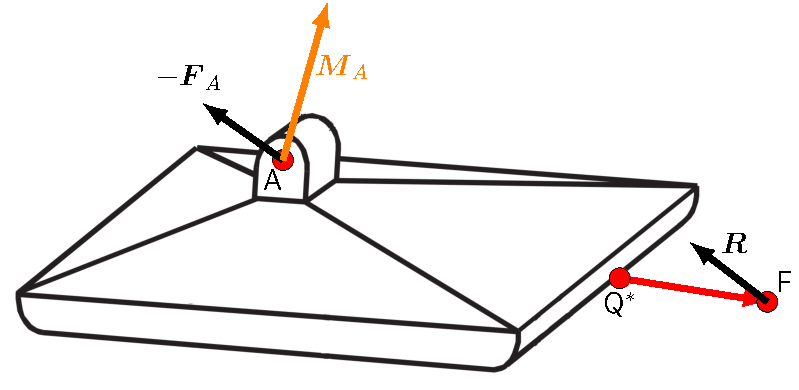
\includegraphics[scale=0.56]{fri}
  \caption{Unstable unbalance. Image edit from \cite{Vukobratov2004}. \label{fig:fri}}
\end{figure}
However the more important result of the introduction of the FRI point can be summarized in the
following principle \cite{Goswami1999}:
\begin{principle}
  The position of the FRI point $F$ is inside the convex hull of the foot support area ($\Omega$)
  IFF the robot is in dynamic equilibrium.
  \[
  F \in \bar{\Omega} \longleftrightarrow \text{dyanamic equilibrium}
  \]
  \par
  It is also possible define the stability margin against the foot rotation.
  It can be  quantified by the minimum distance bewteen the boundary of the support polygon
  $\partial \Omega$ and the location of the FRI point within the sole.
  \par
  Instead, when the FRI point is outside the convex hull of the foot support area the
  $\norm{\vec{QF}}_2$ is a measure of the robot instability.
\end{principle}
At this point it is interesting compare the concept of CoP, ZMP and FRI (FZMP)
underling the difference between the CoP and the ZMP.
\par
In the Figure (\ref{fig:fri_example}) different scenarios are presented. In the first one (a) a
stable gait is illustrated, and the Zero Momentum Point coincides with the CoP. However if
the FZMP (FRI point) is outside the support polygon (b) the ZMP is not defined and the CoP belongs
to the boundary of the support polygon ($\partial \Omega$).
\begin{figure}[!ht]
  \centering
  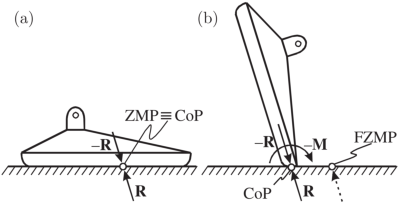
\includegraphics[scale=1.2]{fri_examples}
  \caption{Unstable unbalance. Image taken from \cite{Vukobratov2004}. \label{fig:fri_example}}
\end{figure}
The following conclusions can be done; in the case of the dynamically balanced gait the ZMP always
coincides with the CoP and with the FRI point;
however in the dynamically unbalanced gait  the ZMP is not defined, thus the CoP and
ZMP cannot coincide, also, in this case, the CoP and the FRI point cannot coincide because the
first one must be belong to the foot support area ($\Omega$).
\newpage
